%-------------------------------------------------------------------------------
% seq24_patterns_panel
%-------------------------------------------------------------------------------
%
% \file        seq24_patterns_panel.tex
% \library     Documents
% \author      Chris Ahlstrom
% \date        2015-07-19
% \update      2015-07-19
% \version     $Revision$
% \license     $XPC_GPL_LICENSE$
%
%     Provides the concepts.
%
%-------------------------------------------------------------------------------

\section{Patterns Panel}
\label{sec:seq24_patterns_panel}

   The \textsl{Seq24 Patterns Panel} is the main window of \textsl{Seq24}.
   See \figureref{fig:seq24_main_screen}.

   For exposition, we break it into a top panel, a pattern panel, and a
   bottom panel.    Note that the \textsl{Seq24} main menu is discussed in
   \sectionref{sec:seq24_menu}.

   TODO

\subsection{Patterns, Top Panel}
\label{subsec:seq24_patterns_panel_top}

   TODO

\begin{figure}[H]
   \centering 
   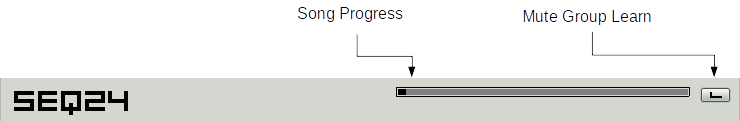
\includegraphics[scale=0.75]{pattern-window-top-panel-items.png}
   \caption{Patterns Panel, Top Panel Items}
   \label{fig:pattern_window_top_panel_items}
\end{figure}

   TODO

\subsection{Patterns, Main Panel}
\label{subsec:seq24_patterns_panel_main}

   The main panel of the Patterns window provides a grid of empty boxes.

\begin{figure}[H]
   \centering 
   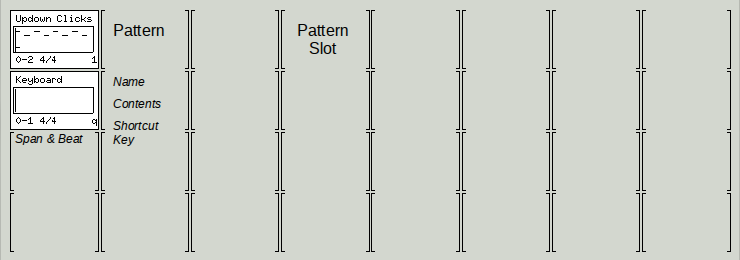
\includegraphics[scale=0.75]{pattern-window-main-panel-items.png}
   \caption{Patterns Panel, Main Panel Items}
   \label{fig:pattern_window_main_panel_items}
\end{figure}

   Each box represents a loop or pattern.
   \index{pattern!right click}
   By right-clicking on an empty box you bring up a menu to create
   a new loop.

\begin{figure}[H]
   \centering 
   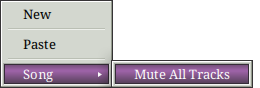
\includegraphics[scale=1.0]{pattern/pattern-empty-right-click-menu.png}
   \caption{Empty Pattern, Right-Click Menu}
   \label{fig:pattern_window_empty_right_click}
\end{figure}

   \begin{enumber}
      \item \textbf{New}
      \item \textbf{Paste}
      \item \textbf{Song / Mute All Tracks}
   \end{enumber}

   \setcounter{ItemCounter}{0}      % Reset the ItemCounter for this list.

   \itempar{New}{pattern!new}
   Creates a new loop or pattern.
   Clicking this menu entry fills in the empty box with an untitled
   pattern, and brings up the Pattern Editor
   so that one can fill in the new pattern.

   \itempar{New}{pattern!paste}
   Pastes a loop or pattern that was previously copied.

   \itempar{Song / Mute All Tracks}{pattern!mute all}
   This item mutes all tracks (or loops/patterns?)





   \index{pattern!right click}
   By right-clicking on an already-filled box you bring up a menu
   or edit a existing one.

\begin{figure}[H]
   \centering 
   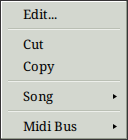
\includegraphics[scale=1.0]{pattern/pattern-right-click-menu.png}
   \caption{Existing Pattern, Right-Click Menu}
   \label{fig:pattern_window_right_click}
\end{figure}

   Right-Clicking will bring up a menu of available options
   for the sequence.  Here you can select the MIDI bus/channel.
   One can also clear all performance data for the pattern (on/off).
   
   TODO: See section [3d] for more info.

   \begin{enumber}
      \item \textbf{Edit...}
      \item \textbf{Cut}
      \item \textbf{Copy}
      \item \textbf{Song/}
      \item \textbf{Midi Bus/}
   \end{enumber}

   \setcounter{ItemCounter}{0}      % Reset the ItemCounter for this list.

   \itempar{Edit}{pattern!edit}
   Edits an existing loop or pattern.
   Clicking this menu entry brings up the Pattern Editor
   so that one can modify the existing pattern.

   \itempar{Cut}{pattern!cut}
   Deletes and copies an existing loop or pattern.

   \textbf{Bug:}
   \index{bugs!pattern cut doesn't work}
   This operation seems to have no effect.  The loop or pattern remains in
   place.

   \itempar{Copy}{pattern!copy}
   Copies an existing loop or pattern.
   The pattern can then be pasted elsewhere in the Patterns panel.

   \itempar{Song}{pattern!song}
   Clicking this menu entry brings up a small popup menu:

\begin{figure}[H]
   \centering 
   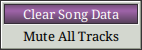
\includegraphics[scale=1.0]{pattern/pattern-menu-song.png}
   \caption{Existing Pattern, Right-Click Menu, Song}
   \label{fig:pattern_window_right_click_song}
\end{figure}

   \begin{enumber}
      \item \textbf{Clear Song Data}
      \item \textbf{Mute All Tracks}
   \end{enumber}

   \setcounter{ItemCounter}{0}      % Reset the ItemCounter for this list.

   \itempar{Clear Song Data}{pattern!clear song data}
   Selecting this filled-box right-click menu item causes that box's
   loop/pattern to be removed from the song.  This means
   that it disappears from the Song Editor window, and so will not
   be played when the song plays.

   \itempar{Mute All Tracks}{pattern!mute all tracks}
   Selecting this filled-box right-click menu item causes...
   TODO.  Cannot yet see that this does anything, NEEDS EXPERIMENTATION.

   \itempar{Midi Bus}{pattern!midi bus}
   Selecting this filled-box right-click menu item brings up a list
   of the 16 MIDI output busses that \textsl{Seq24} supports:

\begin{figure}[H]
   \centering 
   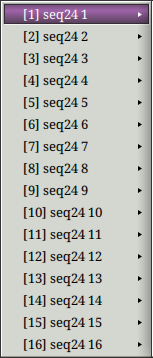
\includegraphics[scale=1.0]{pattern/pattern-menu-midi-bus.png}
   \caption{Existing Pattern, Right-Click Menu, MIDI Bus}
   \label{fig:pattern_window_right_click_midi_bus}
\end{figure}

   For each of these bus items, another pop-up menu allows one
   to specify the MIDI output port for that bus:

\begin{figure}[H]
   \centering 
   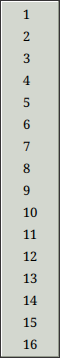
\includegraphics[scale=1.0]{pattern/pattern-menu-midi-bus-numbers.png}
   \caption{Existing Pattern, Right-Click Menu, MIDI Bus Ports}
   \label{fig:pattern_window_right_click_midi_bus_numbers}
\end{figure}




   \index{pattern!left click}
   Left-clicking on a pattern-filled box will change its state
   \index{pattern!mute}
   \index{pattern!unmute}
   from muted (white) to playing (black) when
   the sequencer is running.

   \index{pattern!mute toggle}
   Left-clicking on a Tracks will toggle its playing
   status.  Hitting its assigned keyboard key will
   also toggle its status.  Below is the grid that is
   mapped to the loops/patterns on the screen set.

   \begin{verbatim}
      [1    ][2    ][3    ][4    ][5    ][6    ][7    ][8    ]
      [q    ][w    ][e    ][r    ][t    ][y    ][u    ][i    ]
      [a    ][s    ][d    ][f    ][g    ][h    ][j    ][k    ]
      [z    ][x    ][c    ][v    ][b    ][n    ][m    ][,    ]
   \end{verbatim}

   These characters are shown in the lower right corner of each
   pattern, as an aid to memory.

   \index{pattern!left ctrl click}
   Holding down 'Left Ctrl' while selecting a sequence 
   will mute all other sequences and turn on the selected
   sequences.

   \index{pattern!left click-drag}
   By clicking and holding the left button on a sequence,
   you can drag it to a new location on the grid.  The box
   will disappear while dragged, and reappear in the new location when
   dropped.

   HERE HERE HERE



\subsection{Patterns, Bottom Panel}
\label{subsec:seq24_patterns_panel_bottom}

   TODO

\begin{figure}[H]
   \centering 
   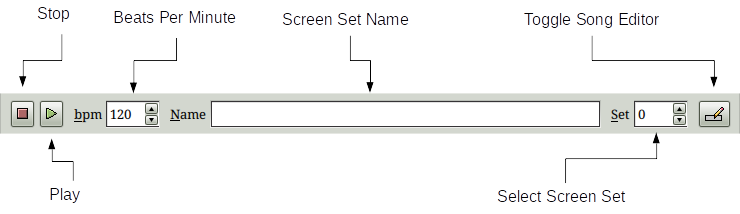
\includegraphics[scale=0.75]{pattern-window-bottom-panel-items.png}
   \caption{Patterns Panel, Bottom Panel Items}
   \label{fig:pattern_window_bottom_panel_items}
\end{figure}

   TODO


%-------------------------------------------------------------------------------
% vim: ts=3 sw=3 et ft=tex
%-------------------------------------------------------------------------------
